\documentclass[crop=false,a4paper,oneside,11pt]{standalone}
\usepackage{a4wide,graphicx,fancyhdr,amsmath,amssymb,float,graphicx,color,geometry,xcolor,titlesec,colortbl,tabu}
\usepackage[parfill]{parskip}
\usepackage[nodayofweek]{datetime}
%----------------------- Macros and Definitions --------------------------

%fast change of things
\newcommand{\mysubject}{2IO70 DBL Embedded Systems}
\newcommand{\myassignment}{Group 12}

%\definecolor{titlepagecolor}{cmyk}{1,.60,0,.40}
%\definecolor{namecolor}{cmyk}{1,.50,0,.10}


\setlength\headheight{20pt}
\addtolength\topmargin{-10pt}
\addtolength\footskip{20pt}

% Define light and dark Microsoft blue colours
\definecolor{MSBlue}{rgb}{.204,.353,.541}
\definecolor{MSLightBlue}{rgb}{.31,.506,.741}
\arrayrulecolor{MSLightBlue}

% Set formats for each heading level

\titleformat*{\section}{\Large\bfseries\sffamily\color{MSBlue}}
\titleformat*{\subsection}{\large\bfseries\sffamily\color{MSLightBlue}}

%date format
\newdateformat{mydate}{\monthname[\THEMONTH] \THEYEAR}

\fancypagestyle{plain}{%
\fancyhf{}
\renewcommand{\headrulewidth}{0pt}
\renewcommand{\footrulewidth}{0pt}
}

\pagestyle{fancy}
\fancyhf{}
\fancyfoot[CO] {\thepage}
\renewcommand{\headrulewidth}{0pt}
\renewcommand{\footrulewidth}{0pt}


%--------------------------------- Text ----------------------------------
\setcounter{secnumdepth}{0}
\begin{document}

\section{Experimental Evaluation}

We ran all the tests in our experimental evaluation on a HP EliteBook 8570w with an Intel i7-3630QM CPU @ 2.40GHz and 8,00 GB RAM. To measure the amount of time and algorithm we start a timer in the code just before the part we want to test and we stop the timer right after the part stops. For testing the 2-position, 4-position and 1-slider algorithms we generated test cases with $5$ different distributions. These distributions are:
\begin{enumerate}
    \item Uniform. Points are randomly placed on a $10000$ by $10000$ plane.
    \item Clustered. Points are placed around $20$ randomly chosen points.
    \item H Clustered. Points are placed around $10$ randomly chosen $y$-coordinates.
    \item V Clustered. Points are placed around $10$ randomly chosen $x$-coordinates.
    \item Bounded. Points are randomly placed on a $1000$ by $1000$ plane.
\end{enumerate}

\subsection{2-position}
\subsubsection{Results}
The algorithm of 2-position model has been explained in the previous section. As a recap, this algorithm has two phase: first we map all the collisions of every candidates of every single point, then we try to place the candidates that has least amount of collisions. For the experimental evaluation of the 2-position algorithm we use $2500$ different test cases with $500$ cases for each distribution. We can show you a example of our results. You can see from figure ..., the solution is quite optimal, we have tried to place as many labels as we can.(Red points mean there are no labels can be placed). 

\begin{figure}[h!]
 \centering
  \centerline{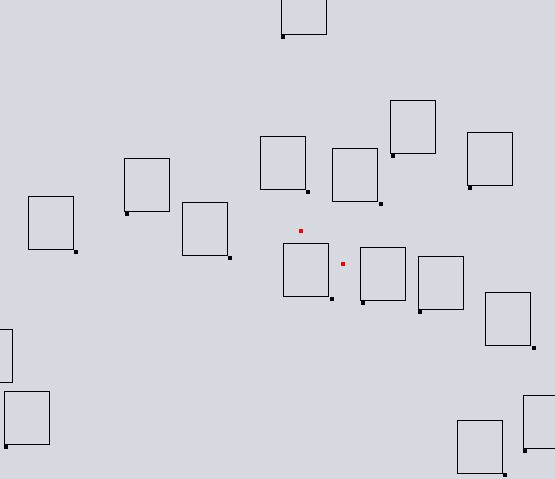
\includegraphics[scale = 0.4]{2pos_example.JPG}}
  \caption{A example of label placement of 2-position model}
 \end{figure} 

\begin{figure}[h!]
 \centering
  \centerline{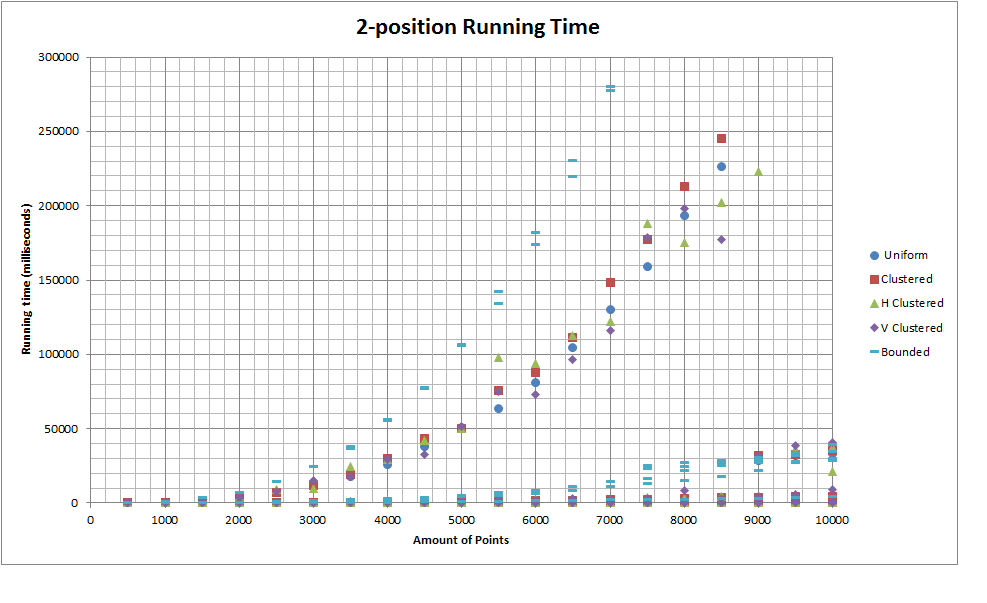
\includegraphics[scale = 0.6]{2PosRunningTime.png}}
  \caption{A graphic showing the running time of the 2-position algorithm}
 \end{figure}

\begin{figure}[h!]
 \centering
  \centerline{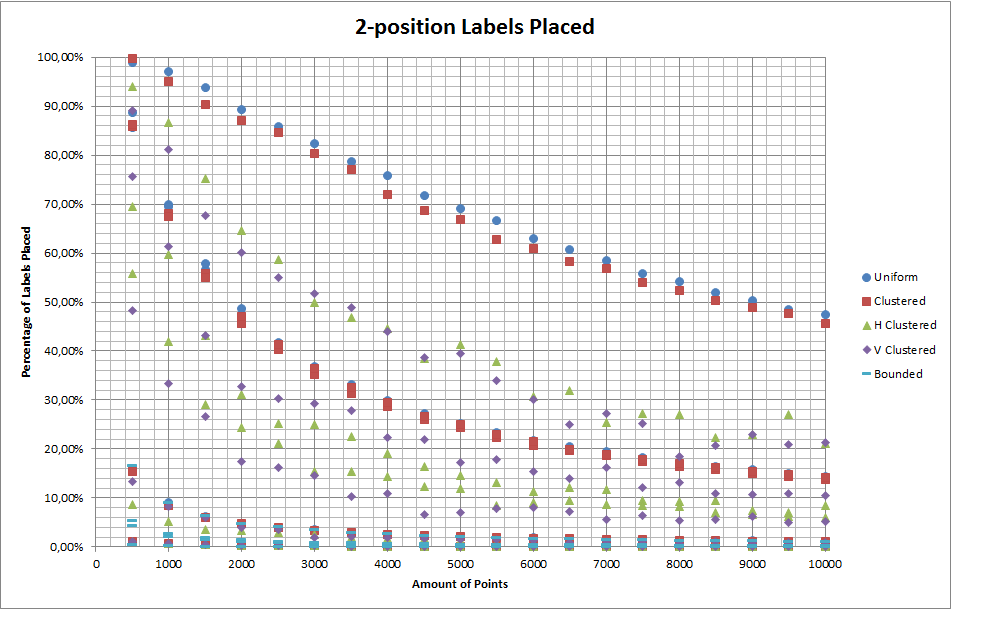
\includegraphics[scale = 0.6]{2PosLabelsPlaced.png}}
  \caption{A graphic showing the percentage of labels placed by the 2-position algorithm}
 \end{figure}
\subsubsection{Discussion}
As we explained in the previous section the theoretical running time of the 2-position algorithm is $O(n^2)$. In figure ..., it shows the running time of $2500$ different cases. You can see most of the cases are quite low in the running time and also close to their best cases. This is because the amount of collisions of the candidates is small, so it will not take much time to map the collisions and it will take less time to place the labels. There are some cases that have higher running time than the others. And we can see from the figure that the practical worst case running time are close to the theoretical running time $O(n^2)$ as we explained before. \\
The worst cases of each distribution suddenly drops when the number of points reaches a specific amount. This is because in these cases, there are too many collisions. If we use the regular algorithm, the running time will become really high so it's not efficient. So in that case, we use greedy algorithm to place the labels. The running time will become lower and the solution is as optimal when using the regular algorithm since there are a lot of collisions.\\
Other than running time, we also look at the amount of placed labels of our algorithm. As we can see from figure ..., when the amount of points are small, the algorithm gives solutions with high percentage of placed labels. When the amount of points become higher, the percentage of placed labels will become lower. This is normal as the labels have the same height and the same width for the same type of distribution but with a higher amount of points. The reason why bounded cases have low solution is because all points are placed in a small area.\\

\subsection{4-position}
\subsubsection{Results}
The algorithm of 4-position model is basically the same as the algorithm of 2-position except it can place two more labels. For the experimental evaluation of the 4-position algorithm we also use $2500$ different test cases with $500$ cases for each distribution. We can also show you an example of our results for 4-position model. You can see from figure ..., the solution is quite optimal, we have tried to place as many labels as we can.(Red points mean there are no labels can be placed).

\begin{figure}[h!]
 \centering
  \centerline{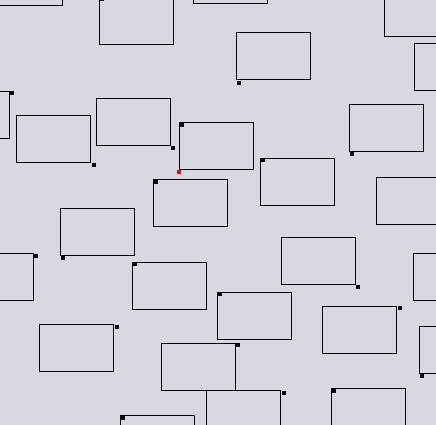
\includegraphics[scale = 0.4]{4pos_example.JPG}}
  \caption{A example of label placement of 4-position model}
 \end{figure}

 \begin{figure}[h!]
 \centering
 \centerline{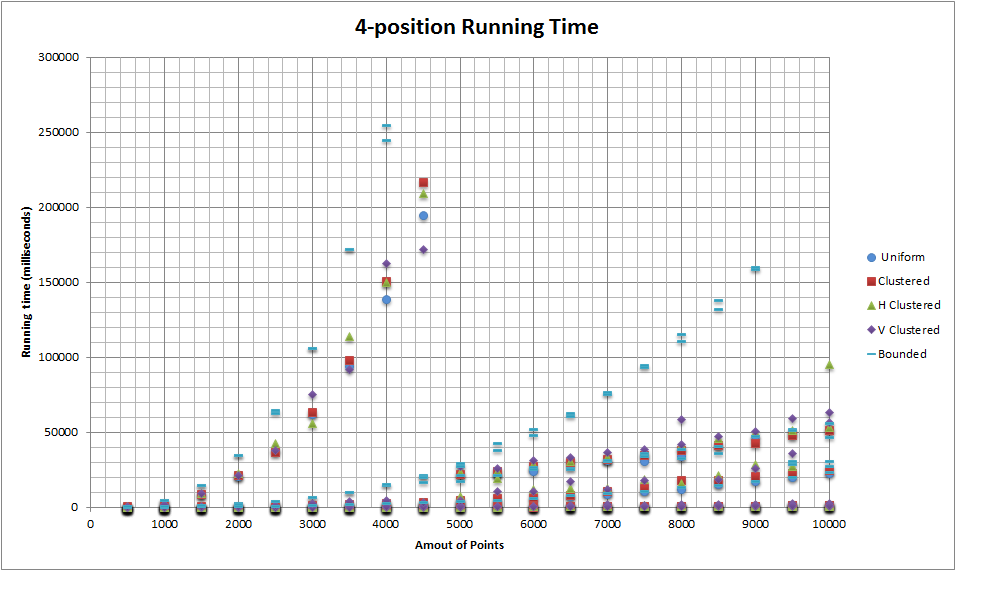
\includegraphics[scale = 0.6]{4PosRunningTime.png}}
 \caption{A graphic showing the Running Time of the 4-position algorithm}
 \end{figure}

 \begin{figure}[h!]
 \centering
  \centerline{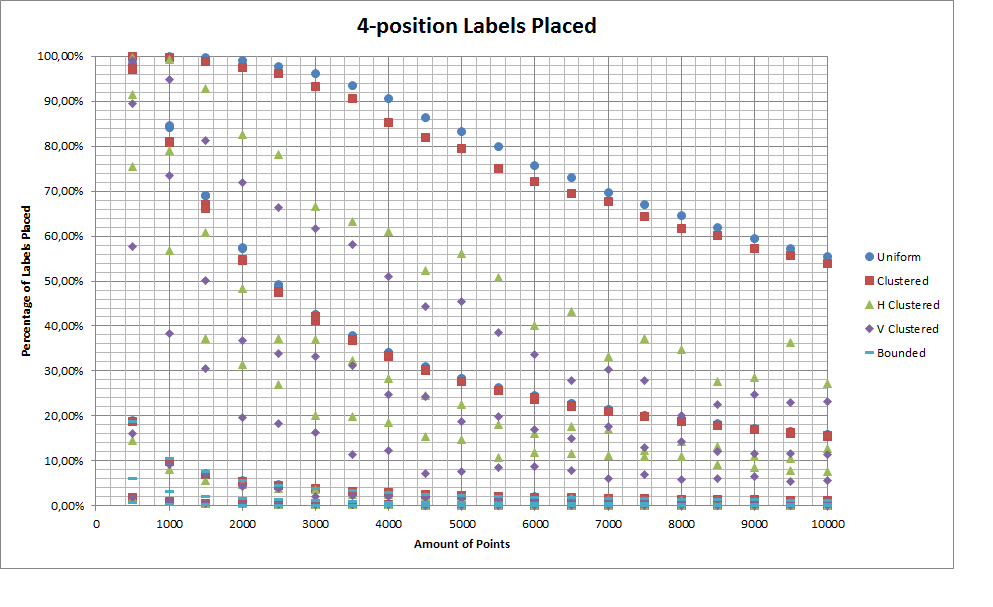
\includegraphics[scale = 0.6]{4PosLabelsPlaced.png}}
  \caption{A graphic showing the percentage of labels placed by the 4-position algorithm}
 \end{figure}
\subsubsection{Discussion}
As we said, the algorithm of 4-position model is nearly the same as the algorithm of 2-position model. Hence the theoretical running time of the 4-position algorithm is also $O(n^2)$. In figure ..., it shows the running time of $2500$ different cases. You can see most of the cases are quite low in the running time and also close to their best cases. This is because the amount of collisions of the candidates is small, so it will not take much time to map the collisions and it will take less time to place the labels. This also happened in our 2-position algorithm. There are some cases that have higher running time than the others. And we can see from the figure that the practical worst case running time are close to the theoretical running time $O(n^2)$. \\
You can see the worst cases of each distribution suddenly drop when the number of points reaches a specific amount as well. This is because in these cases, there are too many collisions. Like in the 2-position algorithm, we use greedy algorithm to place the labels. But there are still some differences between 2-position model and 4-position model. In 4-position algorithm, the worst case running time drop faster than in 2-position algorithm. That's because in 4-position model, there are much more collisions occur between the candidates of labels since it has four labels to place while 2-position only has two.\\
Other than running time, we also look at the amount of placed labels of our algorithm. As we can see from figure ..., when the amount of points are small, the algorithm gives solutions with high percentage of placed labels. When the amount of points become higher, the percentage of placed labels will become lower. This can be explained by the same situation in 2-position model. Compared to the result of 2-position algorithm, 4-position algorithm has higher solution in the percentage of placed labels since it has two more labels to place.\\

\subsection{1-slider}
\subsubsection{Results}
The running time of the 1-slider algorithm can be seen in figure ... We found in practice that the running time of the 1-slider algorithm can exceed the time limit we had of 5 minutes when the amount of overlaps was large. We thus put a hard limit of 4.5 minutes on the heuristic algorithm and, if the algorithm had not given a result by then, ran a greedy algorithm.

The percentage of labels placed by the 1-slider algorithm can be seen in figure ...
\subsubsection{Discussion}

\end{document}
